\section{System Architecture}
\label{evaluation-sec-design}

% 17 Apr 2006 : GWA : Brief overview of system design.  For now I'm going to
%               defer as many details as possible to the evalution sections
%               since we've covered this in some detail in the IEEE article.
%               Also trying to avoid recycling the wording.  I'm working from
%               the paper copy so the skeleton might be similar though.

In this section we provide a brief overview of the design of our volcano
monitoring sensor network and details of the deployment at Reventador. In an
earlier magazine article~\cite{volcano-ieeeic06} we describe the system and
deployment in more detail, although we have not previously published results
evaluating its performance.

\subsection{Sensor hardware}
\label{evaluation-sec-hardware}

\begin{figure}[t]
\label{evaluation-fig-station}
\begin{center}
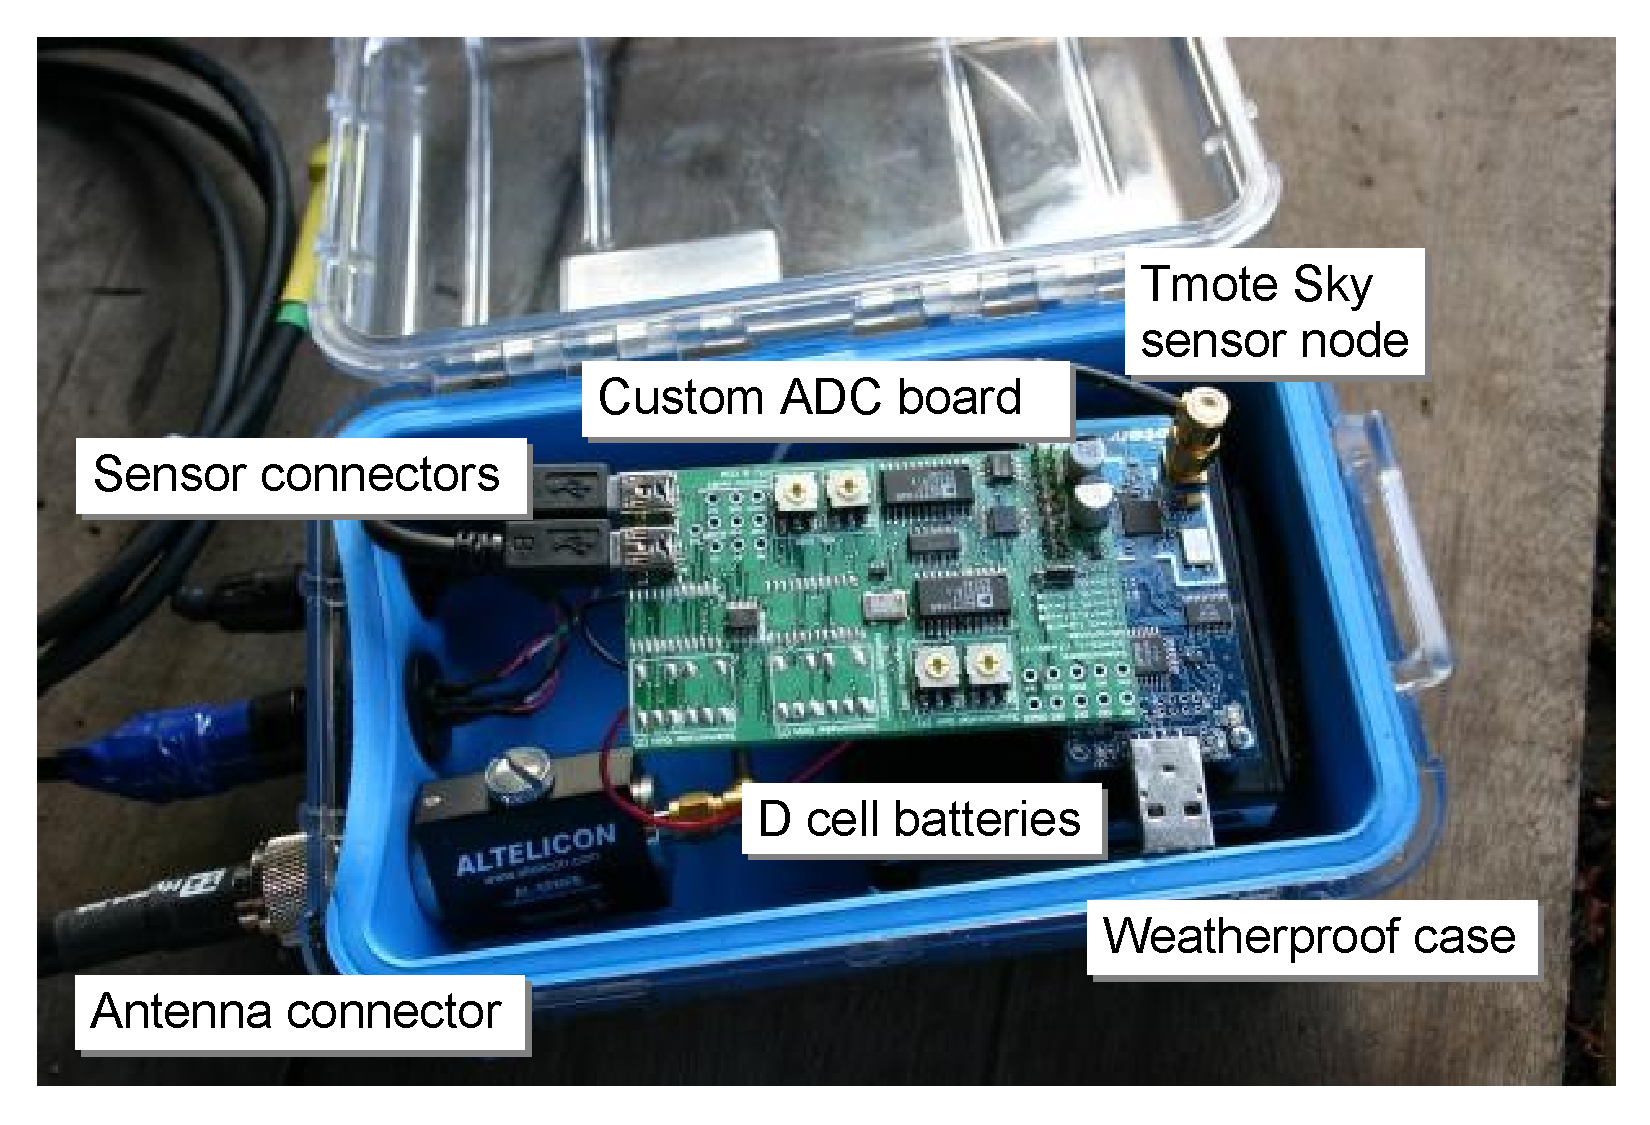
\includegraphics[width=1.0\hsize]{./5-evaluation/figs/pics/Station2-small.pdf}
\end{center}
\caption{\textbf{Our wireless volcano monitoring sensor node.}}
\end{figure}

%We deployed 16 wireless monitoring stations onto Volc\'{a}n Reventador.
%Nodes were arranged in a roughly-linear configuration radiating from the vent
%and spanning over 3km.  Figure REFERENCE shows the locations of each node as
%well as those of several wired monitoring stations deployed nearby.
%\GWAnote{Do we event want to include this figure again? It takes up a lot of
%space but it probably would be nice to have...}

Our wireless sensor node (Figure~\ref{evaluation-fig-station}) is based on
the TMote Sky~\cite{moteiv} platform, which integrates a TI~MSP430 processor,
10~KB of SRAM, 48~KB of program ROM, 1~MByte of flash memory, and a Chipcon
CC2420 radio. All software is implemented in TinyOS~\cite{tinyos-asplos00}.
We designed a custom sampling board that provides four channels of 24-bit
analog-to-digital conversion (TI~AD7710). 
%While the MSP430 provides several channels of ADC, its resolution of 16~bits
%was inadequate for our needs.

Nodes were interfaced to either a single-axis seismometer (GeoSpace GS-11) or
three seismometers in a triaxial configuration (GeoSpace GS-1). 
%The GS-11 sensors are inexpensive and lightweight, but are only sensitive at
%frequencies above 4.5~Hz. In contrast, the GS-1 sensors have a corner
%frequency of 1~Hz but are significantly more expensive and heavy. 
Both sensors are passive instruments; ground motion generates a voltage which
is amplified and digitized by the sampling board.  In addition, each node was
attached to an omnidirectional microphone (Panasonic WM-034BY). This
microphone has been used in other infrasonic monitoring
studies~\cite{johnson-etal-04b}.

% MDW: Node 204 talked to 206 which was 1055 meters away!
Each node was equipped with an 8.5~dBi omnidirectional antenna mounted on
1.5~m of PVC pipe.  This permitted line-of-sight radio range of over 1~km
without amplification; nodes were typically placed 200-400~m apart in our
deployment. Nodes were powered by two D-cell batteries with a lifetime of
approximately 1~week.  Each node was enclosed in a weatherproof Pelican case.

Several other pieces of hardware complete the system. FreeWave radio modems
provided a long-distance radio link between the sensor array and the volcano
observatory, 4.6~km away. A laptop located at the observatory logged data and
was used to monitor and control the network.  Finally, to establish a global
timebase, we used a single Crossbow MicaZ~\cite{xbow} mote interfaced to a
GPS receiver (Garmin OEM~18~LVC).  The GPS receiver provided a 1~Hz pulse
that is accurate to GPS time within 1~$\mu$s, and acted as the root of the
network time synchronization protocol as described in
Section~\ref{evaluation-sec-timing}.

\subsection{Network topology and status monitoring}

Nodes form a multihop routing tree rooted at the gateway node that is
physically attached to the FreeWave modem; we use a variant of
MintRoute~\cite{awoo-multihop} that uses the CC2420's Link Quality Indicator
metric to select routing paths. Each node transmits a {\em status message}
every 10~sec that includes its position in the routing tree, buffer status,
local and global timestamps, battery voltage, and other information. 
%These status messages form the basis of much of the analysis in this paper.
In addition, the base station can issue a {\em command} to each node,
instructing it to respond with an immediate status message, start or stop
data sampling, and set various software parameters.  Commands are propagated
using a simple flooding protocol.  The {\em Deluge} protocol~\cite{deluge}
was also used to permit over-the-air reprogramming and rebooting of nodes.

\subsection{Event detection and data collection}

Because of the high data rates involved (600-1200~bytes/sec from each node)
it is infeasible to continuously transmit all sensor data. Rather, nodes are
programmed to locally detect interesting seismic events and transmit event
reports to the base station. If enough nodes trigger in a short time
interval, the base station attempts to download the last 60~sec of data from
each node.  This design forgoes continuous data collection for increased
resolution following significant seismic events, which include earthquakes,
eruptions, or long-period (LP) events, such as tremor.  The download window
of 60~sec was chosen to capture the bulk of the eruptive and earthquake
events, although many LP events can exceed this window (sometimes lasting
minutes or hours).  To validate our network against existing scientific
instrumentation, our network was designed for high-resolution signal
collection rather than extensive in-network processing.
%In the future we would like to explore more advanced in-network signal
%processing.

During normal operation, each node continuously samples its seismic and
acoustic sensors at 100~Hz, storing the data to flash memory. Data is stored
as 256-byte {\em blocks} in the flash.
%with each block identified by a monotonically increasing {\em block ID}.
Each block 
%is tagged with its ID 
is tagged with the {\em local timestamp} corresponding to the first sample in
the block.  This timestamp is later mapped onto a global time reference as
described in Section~\ref{evaluation-sec-timing}. The 1~Mbyte flash is
treated as a circular buffer storing approximately 20~min of data. 

In addition, nodes run an {\em event detection algorithm} that computes two
exponentially-weighted moving averages (EWMA) over the input signal with
different gain settings. When the ratio between the two EWMAs exceeds a
threshold, the node transmits an event report to the base station.
%$\alpha_{\mathit{high}} > \alpha_{\mathit{low}}$.  That is, the high-gain
%EWMA is more sensitive to changes in the input signal than the low-gain
%EWMA. If the ratio of the high-gain EWMA to the low-gain EWMA exceeds a
%threshold $T$, the node considers the signal to contain a significant event
%and transmits a {\em trigger} message to the base station.
If the base station receives triggers from 30\% of the active nodes within a
10~sec window, it considers the event to be well-correlated and initiates
data collection.

Our reliable bulk-transfer protocol, called {\em Fetch}, operates as follows.
The base station waits for 30~sec following an event before iterating through
all nodes in the network. The base sends each node a command to temporarily
stop sampling, ensuring the event will not be overwritten by subsequent
samples.  For each of the 206~blocks in the 60~sec window, the base sends a
{\em block request} to the node.  The node reads the requested block from
flash and transmits the data as a series of 8~packets.  After a short timeout
the base will issue a repair request to fill in any missing packets from the
block.
%The repair process continues until all packets have been received or a
%timeout occurs. 
Once all blocks have been received or a timeout occurs, the base station
sends the node a command to resume sampling and proceeds to download data
from the next node. 
%The data is logged by the base station laptop for later analysis.

\subsection{Deployment on Volc\'{a}n Reventador}

\begin{figure}[t]
\label{evaluation-fig-schematic}
\begin{center}
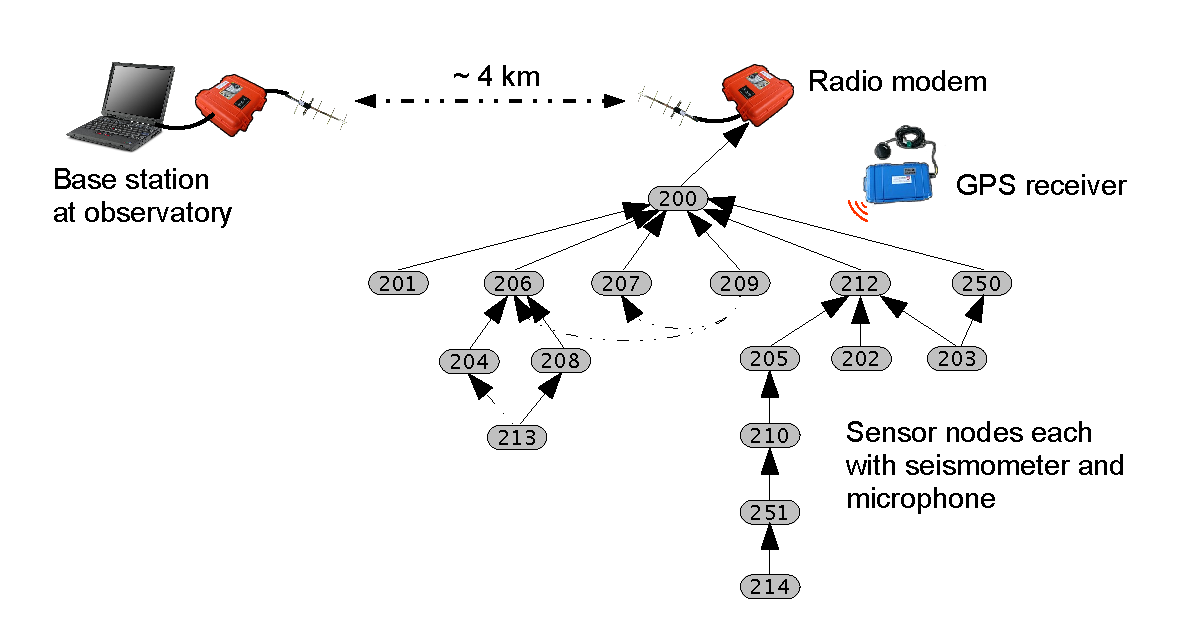
\includegraphics[width=1.0\hsize]{./5-evaluation/figs/pics/schematic2.pdf}
\end{center}
\caption{\textbf{Sensor network architecture.} Nodes form a
multihop routing topology, relaying data via a long-distance radio
modem to the observatory. A GPS receiver is used to establish a global
timebase. The network topology shown here was used during
our deployment at Reventador.}
\end{figure}

\begin{figure}[t]
\label{evaluation-fig-map}
\begin{center}
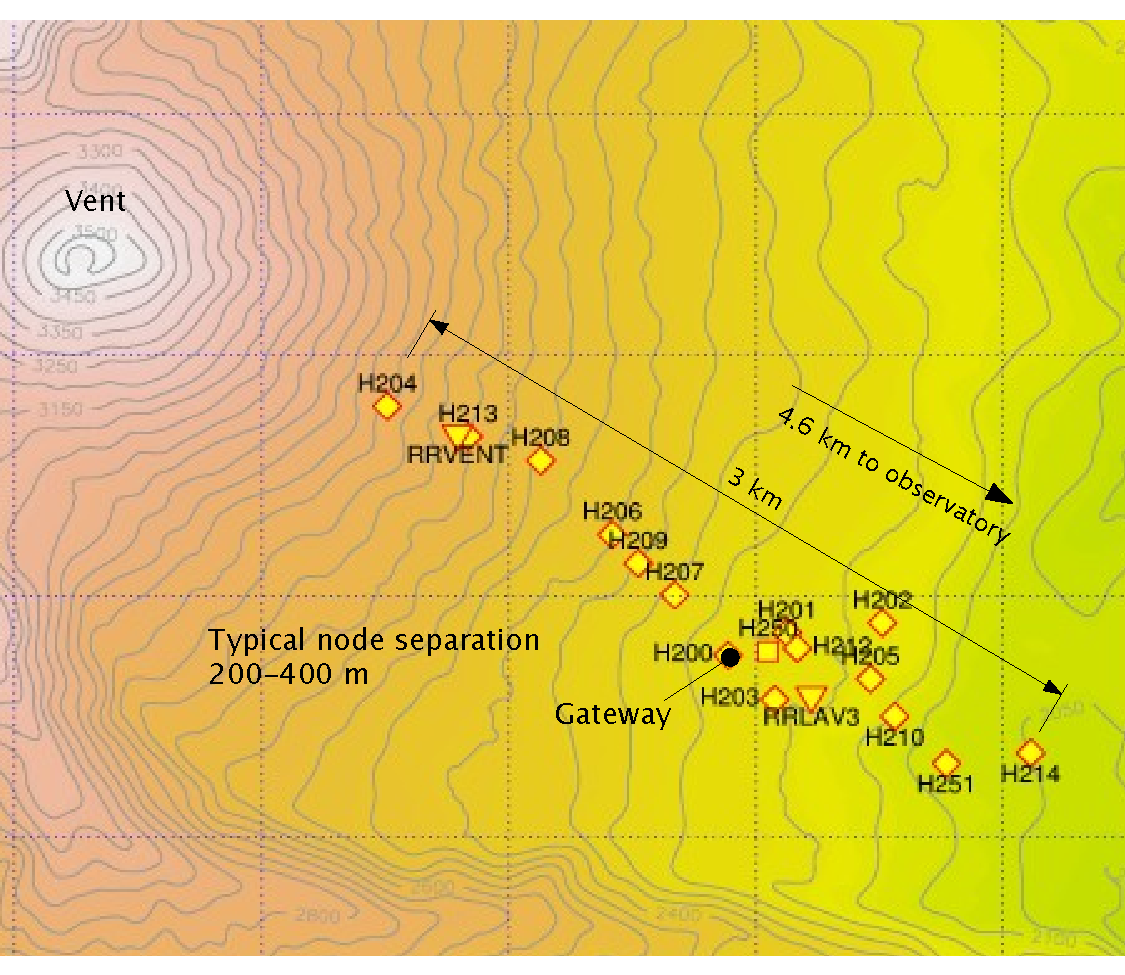
\includegraphics[width=1.0\hsize]{./5-evaluation/figs/pics/reventador-map-crop.pdf}
\end{center}
\caption{\textbf{Map of sensor deployment at Volc\'{a}n Reventador.}
In addition to the 16~sensor nodes, two broadband seismometers
with data loggers (RRVENT and RRLAV3) were colocated with the network.}
\end{figure}

% MDW 26-Aug-06: I have revisited some of Jeff Johnson's suggestions
% in the below text; i.e., hyphenation on "broad-band" and so forth.

Our deployment at Reventador took place between August 1--19, 2005.
Reventador is an active volcano located in northern Ecuador, about 100~km
from Quito. 
%The volcano erupted with massive force in 2002, blanketing the streets of
%Quito with ash, closing schools and the airport. 
During this time, Reventador's activity consisted of small explosive events
that ejected ash and incandescent blocks several times a day. Associated
seismicity included numerous explosion earthquakes as well as
extended-duration shaking (tremor) and shallow rock-fracturing earthquakes.

We deployed 16~sensor nodes on the upper flanks of Reventador, as shown in
Figure~\ref{evaluation-fig-map}, over a 3~km linear configuration radiating
away from the vent. The resulting multihop topology is shown in
Figure~\ref{evaluation-fig-schematic}. The upper flanks of the volcano were
completely deforested by a large eruption in November 2002, allowing for
line-of-sight radio communication between adjacent sensor nodes.  Two
standalone seismic stations, consisting of a broadband sensor, a Reftek 130
data logger with 1~GByte flash memory cards, and a GPS receiver for
timestamping, were colocated with sensor nodes. The data from these stations
is essential to our network validation, described in
Sections~\ref{evaluation-sec-eventdetection}~and~\ref{evaluation-sec-timing}.
The base station was located at a small hotel 4.6~km from the deployment
site.  The sensors were deployed for a total of 19~days, during which time
the network recorded data from 229~earthquakes, eruptions, and tremor events,
logging 107~MBytes of data. The long hike and lack of roads prevented
frequent returns to the deployment site, although we returned several times
to change batteries and perform other network maintenance.

%Colocated with our
%sensor network were two broadband seismometer stations,
%each using a Reftek~130 data logger with 1~GByte flash memory cards
%and a GPS receiver for timestamping. The data from these stations 
%is essential to our network validation, described in 
%Sections~\ref{sec-eventdetection}~and~\ref{sec-timing}.  
%The base station was located at 
%a small hotel 4.6~km from the deployment site. 

% MDW 26-Aug-06: I don't think this subsection is really needed. 
% Maybe the first paragraph could be added back somewhere; the rest is
% not pithy enough to warrant inclusion.

%\subsection{Design decisions}
%
%For this deployment our primary design goals were simplicity,
%statelessness, and robustness.  As such, we chose not to focus on
%aggressive power management, routing performance, fault tolerance
%(e.g. multiple base stations and GPS receivers), or scalability.  We
%plan to address these issues in future deployments.
%
%Some of our design decisions were influenced by the fact that the deployment
%site was a strenuous 3~hour hike from the observatory, meaning that we wanted
%to avoid problems that might require returning to the deployment
%site.  Other decisions were driven by more pragmatic reasons.  For example,
%although having a GPS receiver on each node would make the system more
%robust, we decided against it due to the increased cost, power, and
%deployment logistics.  Each GPS node requires a car battery to power it for a
%longer duration, making the deployment impractical given the difficult
%circumstances.  Instead we decided to equip only one node with a GPS receiver
%and use FTSP~\cite{ftsp} to synchronize the rest of the network.
%
%Finally, we point out that initially we planed on a 25~node network.
%However, because of various hardware failures we ended up with 16
%deployable nodes.

